\chapter{Rust toolchain}

Die Rust toolchain ist eine Sammlung von Werkzeugen, die dabei helfen, den Compiler aktuell zu halten und Projekte zu verwalten.


\section{rustup}

Das Rustup-Tool ist die empfohlene Installationsmethode für Rust. Das Tool ermöglicht zusätzlich die Verwaltung von verschiedenen Versionen, Komponenten und Plattformen. Um zwischen den Versionen stable, beta und nightly zu wechseln, kann auf der Kommandozeile eingegeben werden:

\begin{lstlisting}   
    rustup install beta                 # release channel
    rustup install nightly
    rustup update                       # update all channels
    rustup toolchain default nightly    # switch to 'nightly'
\end{lstlisting}

Rust unterstützt auch das Kompilieren für andere Zielsysteme, dabei kann rustup helfen. So kann man beispielsweise MUSL verwenden:

\begin{lstlisting}
    # add target
    rustup target add x86-64-unknown-linux-musl
    # build project with target
    cargo build --target=x86_64-unknown-linux-musl
\end{lstlisting}

Mit Hilfe von rustup können verschiedene Komponenten installiert werden, z.B.:

\begin{itemize}
    \item rust-docs: Lokale Kopie der Rust-Dokumentation, um sie offline lesen zu können.
    \item rust-src: Lokale Kopie des Quellcodes von Rust. Autokomplettierungs-Tools verwenden diese Information.
    \item rustfmt-preview: Zur automatischen Code-Formatierung.
\end{itemize}

\begin{lstlisting}
    rustup component add rustfmt-preview
\end{lstlisting}


\section{rustc}

Der Compiler von Rust, er übersetzt den Quellcode in einen binären code, entweder als Bibliothek oder als ausführbare Datei. Die meisten Rust-Programmierer rufen rustc nicht direkt auf, sondern indirekt über Cargo.

\subsection{Grundlegende Verwendung}

Der Kommandozeilenbefehl für das Kompilieren mit rustc ähnelt dem eines C-Programms:

\begin{lstlisting}
    gcc   hello.c  -o helloC            # C program
    rustc hello.rs -o helloRust         # Rust program
\end{lstlisting}

Anders als in C muss nur der crate root\footnote{Quellcode-Datei mit der main() Methode} angegeben werden. Der Compiler kann mithilfe des Codes selbständig festellen, welche Dateien er übersetzen und linken muss. Es müssen somit keine Objektdateien erstellt werden.

\subsection{Lints}

Ein Lint ist ein Werkzeug, das zur Verbesserung des Quellcodes verwendet wird. Der Rust-Compiler enthält eine Reihe von Lints. Beim Kompilieren werden dadurch Warnungen oder Fehlermeldungen ausgeben. Beispiel:

\begin{lstlisting}
    $ cat main.rs
    fn main() {
        let x = 5;
    }

    $ rustc main.rs
    warning: unused variable: `x`
     --> main.rs:2:9
      |
    2 |     let x = 5;
      |         ^ help: consider using `_x` instead
      |
      = note: #[warn(unused_variables)] on by default
\end{lstlisting}

Das ist das \glqq unused\_variables\grqq{} Lint. Es besagt, dass eine Variable eingeführt wurde, die nicht im Code verwendet wurde. Dies ist nicht falsch, es könnte jedoch ein Bug sein.


\section{Cargo}

Cargo ein Projektmanager für Rust. Damit können Abhängigkeiten heruntergeladen und verteilbare Pakete erstellt werden, welche auf crates.io\footnote{Paketeregister der Rust-Community} hochgeladen werden können.

\subsection{Projektverwaltung}

Projekte können mit Hilfe von Cargo erstellt werden, dabei entsteht eine bestimmte Ordnerstruktur mit einer Cargo.toml Datei sowie dem crate root im src-Ordner. Ein Projekt kann eine Applikation (binary) oder eine Bibliothek (library) sein. Der crate root ist bei einer Applikation immer \glqq main.rs\grqq{} und bei einer Bibliothek \glqq lib.rs\grqq{}.

\begin{lstlisting}[style=tree]
    $ cargo new hello_world --bin       # --lib for library
         Created binary (application) `hello_world` package

    $ cd hello_world
    $ tree .
    .
    ├── Cargo.toml
    └── src
        └── main.rs
    
    1 directory, 2 files
\end{lstlisting}

Die Cargo.toml enthält alle wichtigen Metainformationen, die Cargo zum Kompilieren benötigt. 

\begin{lstlisting}
    [package]
    name = "hello_world"
    version = "0.1.0"
    authors = ["Thomas Keck <s-tkeckk@haw-landshut.de>"]
    edition = "2018"
    
    [dependencies]    
\end{lstlisting}

Die Informationen über den Author enthält Cargo von den Umgebungsvariablen CARGO\_NAME und CARGO\_EMAIL. In Rust gibt es sogenannte editions, welche in der Regel in einem zeitlichen Abstand von zwei oder drei Jahren veröffentlicht werden und, ähnlich wie in C, einen Standard festlegen. Zum Zeitpunkt der Erstellung dieser Arbeit gibt es zwei Editionen: 2015 und 2018. Das Pendant in C wären die C-Standards wie z.B. C90, C99 oder C11.

Zudem können hier zusätzliche Bibliotheken angegeben werden, die Cargo automatisch von crates.io herunterlädt in in das Projekt einbindet. Cargo erstellt für genauere Informationen der Abhängigkeiten eine Datei Cargo.lock, diese sollte nicht manuell verändert werden, da sie von Cargo gepflegt wird. Mithilfe von Cargo können Tests gestartet werden, genauere Information dazu sind aus Kapitel 3.6 zu entnehmen.

\subsubsection{Projekt-Layout}

\begin{figure}[htbp]
    \centering
    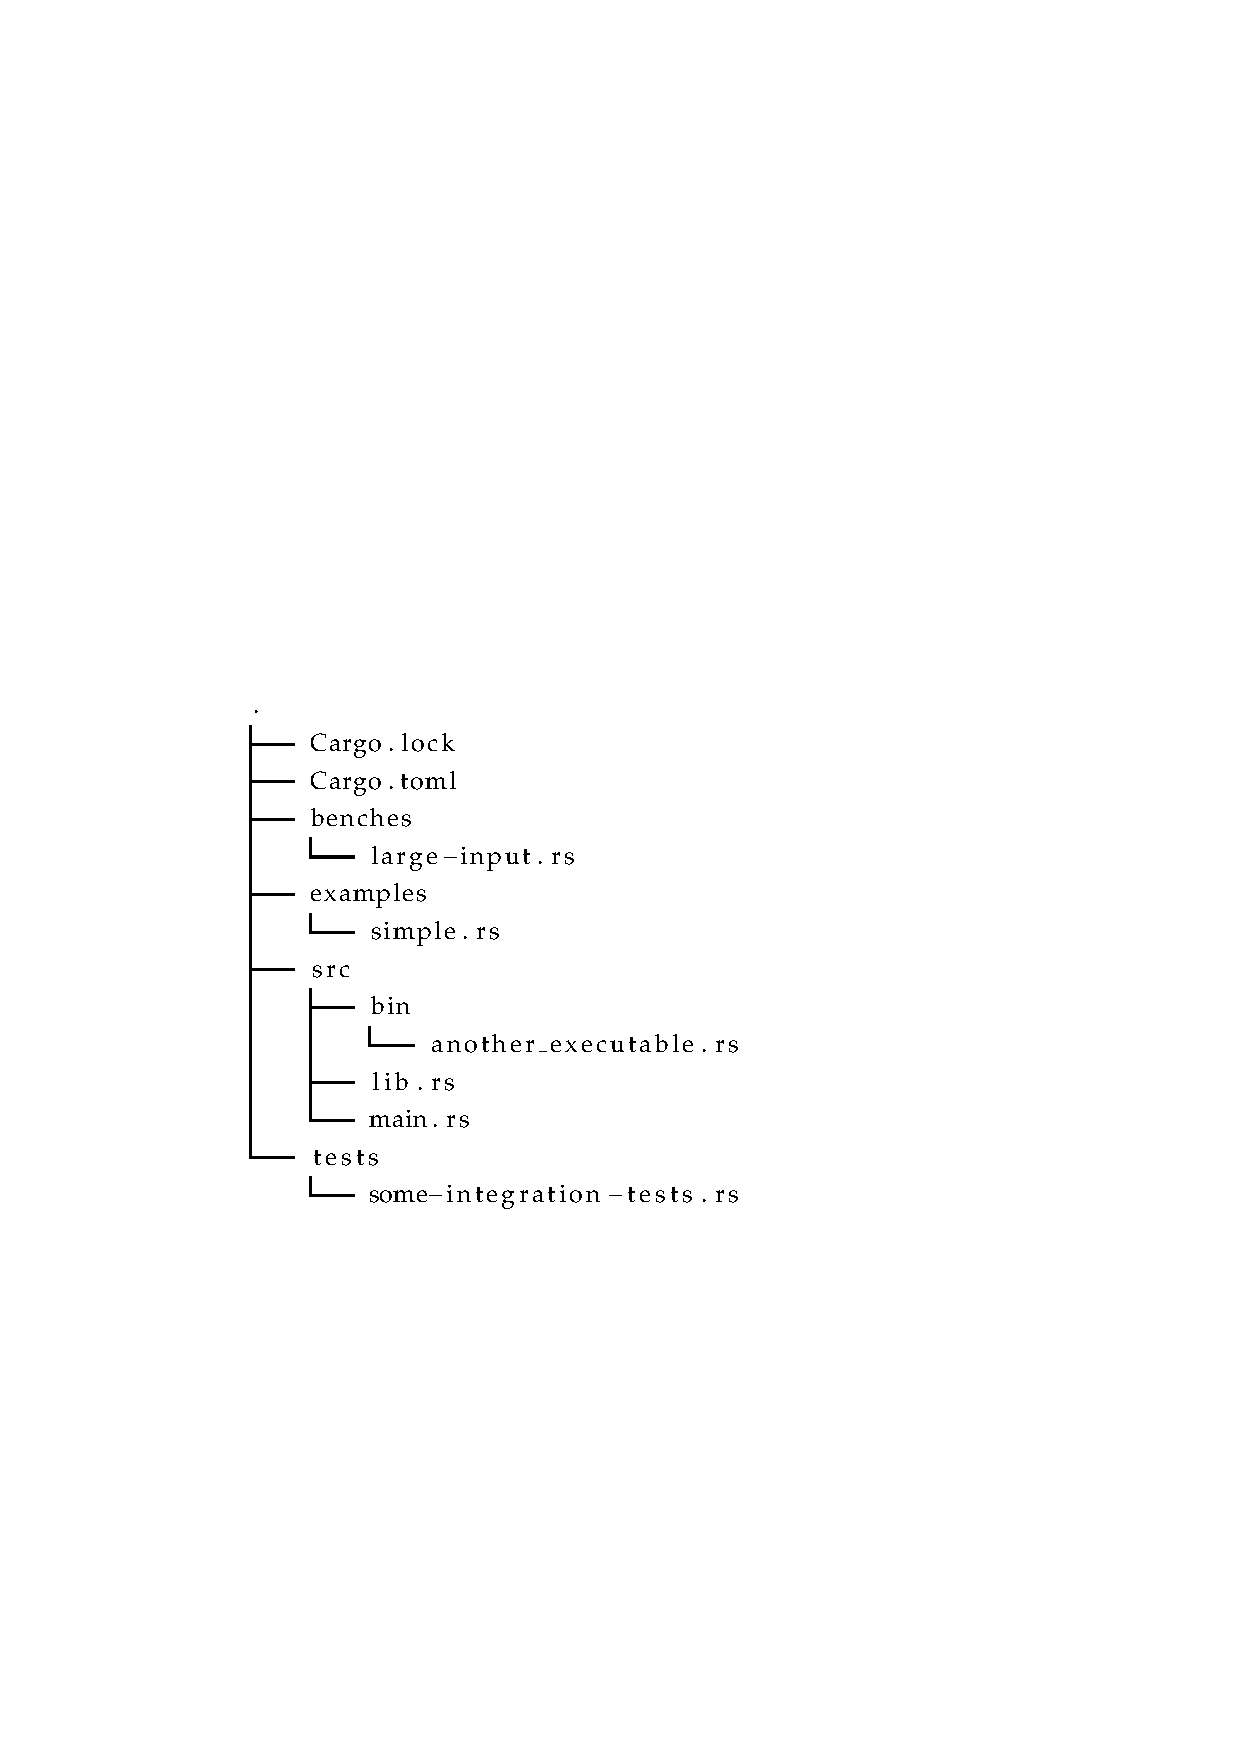
\includegraphics{Toolchain/dateibaum.pdf}
    \caption{Dateibaum eines Rust Projekts}
\end{figure}

\begin{itemize}
    \item Cargo.toml und Cargo.lock werden im Wurzelverzeichnis des Projekts gespeichert
    \item Quellcode-Dateien sind im src-Ordner vorgesehen
    \item Die Standarddatei für Bibliotheken ist src/lib.rs
    \item Die Standarddatei für ausführbare Programme ist src/main.rs
    \item Quellcode für sekundäre ausführbare Programme src/bin/*.rs
    \item Integrationstests im Ordner tests, Unit-Tests werden in die jeweilige Programmdatei geschrieben
    \item Beispiele im examples Ordner
    \item Benchmarks im benches Ordner
\end{itemize}

\subsubsection{Wichtige Kommandozeilenbefehle für Cargo}

Zum Kompilieren uns Ausführen:

\begin{lstlisting}
    $ cargo build
    $ ./target/debug/hello_world

    $ cargo build --release             # optimized performance
    $ ./target/release/hello_world

    # alternative as one command
    $ cargo run
\end{lstlisting}

Zum Testen:

\begin{lstlisting}
    # run all standard tests
    $ cargo test

    # run all tests marked as ignored
    $ cargo test -- --ignored
\end{lstlisting}
